% =====================================================================
%  CN Project, team1: Final Report (IEEE conference format)
%  Build:  tectonic --outdir Docs Docs/report/main.tex   ->  Docs/main.pdf
% =====================================================================
\documentclass[conference,a4paper]{IEEEtran}

\usepackage{fontspec}
\setmainfont{texgyretermes}[Extension=.otf, UprightFont=*-regular, BoldFont=*-bold,
  ItalicFont=*-italic, BoldItalicFont=*-bolditalic]
\setmonofont{Inconsolatazi4}[Extension=.otf, UprightFont=*-Regular, BoldFont=*-Bold, Scale=0.92]
\usepackage{graphicx}
\usepackage{booktabs}
\usepackage{array}
\usepackage{tabularx}
\usepackage{multirow}
\usepackage{xcolor}
\usepackage{listings}
\usepackage{tikz}
\usetikzlibrary{positioning,arrows.meta,shapes.geometric,fit,calc,backgrounds}
\usepackage{float}
\usepackage{cite}
\usepackage{url}
\usepackage[hidelinks]{hyperref}

\definecolor{codebg}{HTML}{F5F6F8}
\definecolor{rule}{HTML}{9AA3AE}
\definecolor{edge}{HTML}{E8830C}
\definecolor{dns}{HTML}{7A4DFF}
\definecolor{bka}{HTML}{14A06A}
\definecolor{bkb}{HTML}{2F6BFF}
\definecolor{old}{HTML}{9AA3AE}
\definecolor{new}{HTML}{14A06A}

\lstset{
  basicstyle=\ttfamily\scriptsize,
  backgroundcolor=\color{codebg},
  frame=tb, rulecolor=\color{rule},
  columns=fullflexible, keepspaces=true,
  breaklines=true, breakatwhitespace=false,
  postbreak=\mbox{\textcolor{rule}{$\hookrightarrow$}\space},
  showstringspaces=false, aboveskip=6pt, belowskip=4pt,
  xleftmargin=2pt, xrightmargin=2pt, captionpos=b
}

\makeatletter\setlength{\@fptop}{0pt}\setlength{\@dblfptop}{0pt}\makeatother
\newcommand{\code}[1]{\texttt{#1}}
\renewcommand{\arraystretch}{1.12}
\newcolumntype{L}{>{\raggedright\arraybackslash}X}
\newcolumntype{P}[1]{>{\raggedright\arraybackslash}p{#1}}

\begin{document}

\title{{\large\begin{tabular}{@{}c@{}}Computer Networks Capstone Project,\\Rishihood University, Sonipat\end{tabular}}\\[4pt]Design, Implementation and Hardening of a\\Private Network Service Platform on Four Laptops}

\author{%
\normalsize
\begin{tabular}{@{}c@{\hspace{1.6em}}c@{\hspace{1.6em}}c@{\hspace{1.6em}}c@{}}
{\large Narendra Singh} & {\large Mohan Kumar C R} & {\large Keshav Rajput} & {\large Mayank Gupta}\\[3pt]
Enrollment No. 2401010292 & Enrollment No. 2401010282 & Enrollment No. 2401010222 & Enrollment No. 2401010267\\
\textit{Edge, LB and TLS (Mac 2)} & \textit{DNS and Client (Mac 1)} &
\textit{Backend A, Standby (Mac 3)} & \textit{Backend B (Mac 4)}\\
\end{tabular}%
}

\maketitle

\begin{abstract}
This report presents the design, implementation, observation and hardening of a fully local
private service platform built by a four-member team on four macOS laptops sharing one campus
Wi-Fi subnet, with no cloud resources. A client resolves the private name
\code{app.team1.test} through the team's own DNS server (dnsmasq), opens a TLS-protected
connection to an nginx edge that terminates TLS with a certificate issued by a team-operated
certificate authority, and is load-balanced round-robin across two minimal REST backends. In
Phase~1 the platform was built and every layer was verified: DNS resolution by two or more
clients, certificate validation without bypass flags (\code{Verify return code: 0}), TLS~1.3
negotiation, A/B alternation visible in an \code{X-Backend} response header, HTTP caching with a
\code{304 Not Modified} revalidation, and five controlled failure scenarios each isolated to a
single layer. In Phase~2 the platform was hardened with a backup DNS resolver (page load
preserved in 2.55~s with the primary stopped), a 30~s TTL experiment, packet-filter isolation of
the backend ports, passive health-check failover, a standby edge with a DNS-based cutover
completed in approximately 28~s, and a layered troubleshooting procedure. The report also
documents the problems met during the work, the evidence collected, and the limitations of the
results.
\end{abstract}

\begin{IEEEkeywords}
DNS, dnsmasq, TLS, public key infrastructure, reverse proxy, nginx, load balancing, HTTP caching,
high availability, packet filtering, network troubleshooting.
\end{IEEEkeywords}

% =====================================================================
\section{Introduction}
A single web request crosses several protocol layers before any application
code runs: a name is resolved, a transport connection is opened, a secure channel is
negotiated, and only then is an HTTP request delivered to a server. The objective of this
course project~\cite{brief} is to make that journey visible by building every component of it
from first principles on hardware the team controls, and then to show how the system behaves
when parts of it fail.

The guiding principle of the project is that \emph{the application stays simple; the network is
the project}. The backend therefore returns small JSON documents, and all effort is placed on
naming, transport, security, load distribution, caching, resilience and diagnosis.

The work was carried out in two phases. Phase~1 (\emph{Build and Observe}) delivers a working
platform and evidence for each layer of a request. Phase~2 (\emph{Harden and Recover}) removes
single points of failure, introduces service isolation, measures the effect of DNS caching on
change propagation, and formalises a troubleshooting method.

The main contributions of this report are:
\begin{itemize}
\item a reproducible four-host architecture with one configuration file as the single source of
truth for addressing (Section~\ref{sec:arch});
\item the Phase~1 implementation and layer-by-layer verification, including five controlled
failures (Sections~\ref{sec:p1} and~\ref{sec:fail});
\item the Phase~2 extensions with measured results and a Phase~2 final report
(Sections~\ref{sec:p2} and~\ref{sec:p2report});
\item a candid account of the difficulties met and the limitations of the evidence
(Sections~\ref{sec:disc} and~\ref{sec:limits}).
\end{itemize}

% =====================================================================
\section{Background}
\label{sec:bg}

\subsection{Domain Name System}
DNS maps names to resource records~\cite{rfc1034,rfc1035}. An \emph{A} record maps a name to an
IPv4 address and carries a time-to-live (TTL) that bounds how long resolvers and clients may
cache it. DNS only answers a lookup; it never carries the application traffic that follows. The
\code{.test} top-level domain is reserved for testing~\cite{rfc2606}; \code{.local} was avoided
because macOS routes it to multicast DNS~\cite{rfc6762}.

\subsection{Transport and Security}
TCP provides a reliable byte stream opened by a three-way handshake
(SYN, SYN-ACK, ACK)~\cite{rfc9293}. TLS authenticates the server and encrypts the
stream~\cite{rfc8446,rfc5246}. Authentication relies on an X.509 certificate chain~\cite{rfc5280}:
the client must trust the issuing certificate authority (CA), the signature must verify, and the
requested host name must appear in the certificate's Subject Alternative Name (SAN) extension.
In TLS~1.3 the server certificate is itself encrypted, whereas in TLS~1.2 it is visible on the
wire.

\subsection{HTTP, Caching and Load Balancing}
HTTP semantics and caching are defined in~\cite{rfc9110,rfc9111}. \code{Cache-Control: max-age}
allows reuse without contacting the server, and an \code{ETag} validator allows a conditional
request (\code{If-None-Match}) to be answered with a body-less \code{304 Not Modified}. A reverse
proxy accepts client connections and forwards requests to a pool of upstream servers; nginx
implements round-robin distribution, passive health checks and request retries in its upstream
and proxy modules~\cite{nginxup,nginxproxy}.

\subsection{Packet Filtering}
The macOS packet filter \code{pf}~\cite{pf} matches packets by protocol, source, destination and
port. A \code{block drop} rule discards packets silently, which a client observes as a timeout;
a closed port without filtering instead returns a TCP reset, observed as an immediate
\emph{connection refused}.

% =====================================================================
\section{System Architecture}
\label{sec:arch}

\subsection{Topology and Roles}
All four laptops joined the same campus Wi-Fi segment, \code{10.7.0.0/19}
(netmask \code{255.255.224.0}, default gateway \code{10.7.0.1}). No device sits between the
laptops at the network layer, so every host reaches every other host directly. Fig.~\ref{fig:topo}
shows the topology and Table~\ref{tab:roles} the role of each machine together with its cloud
equivalent.

\begin{figure*}[t]
\centering
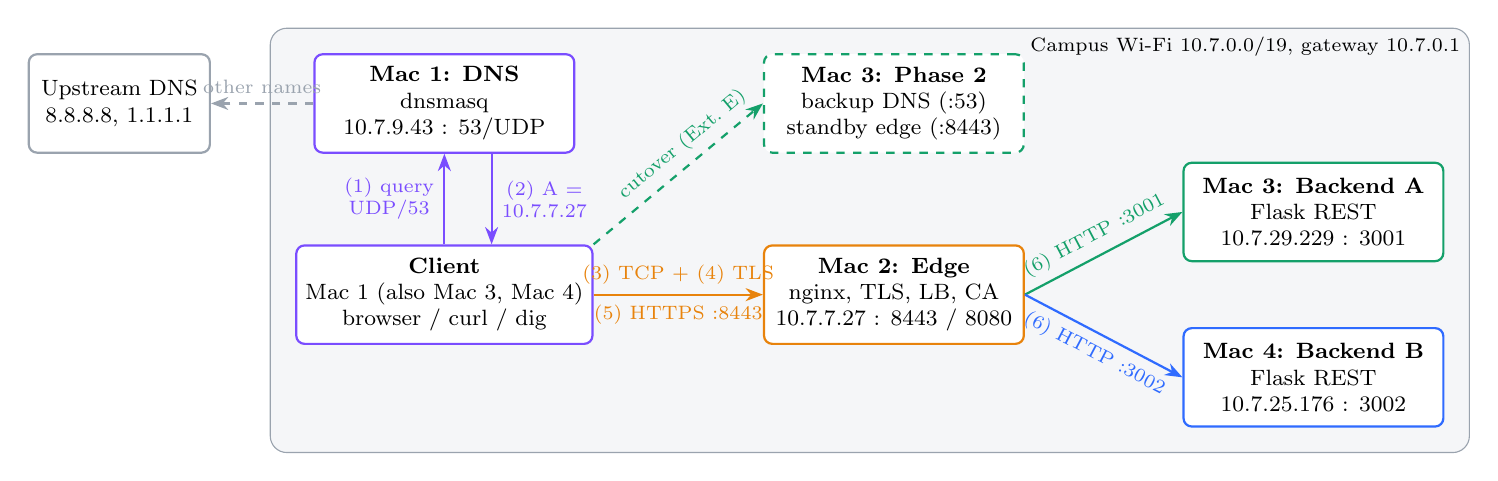
\begin{tikzpicture}[
  font=\footnotesize,
  host/.style={draw, rounded corners=3pt, thick, align=center, minimum width=3.3cm,
               minimum height=1.25cm, fill=white},
  stby/.style={host, dashed},
  lbl/.style={font=\scriptsize, align=center},
  arr/.style={-{Stealth[length=2.2mm]}, thick},
  darr/.style={-{Stealth[length=2.2mm]}, thick, dashed}
]
\node[host, draw=dns] (c) at (0,0) {\textbf{Client}\\Mac 1 (also Mac 3, Mac 4)\\browser / curl / dig};
\node[host, draw=dns, above=1.15cm of c] (dns) {\textbf{Mac 1: DNS}\\dnsmasq\\10.7.9.43 : 53/UDP};
\node[host, draw=edge, right=2.15cm of c] (edge) {\textbf{Mac 2: Edge}\\nginx, TLS, LB, CA\\10.7.7.27 : 8443 / 8080};
\node[host, draw=bka, right=2.0cm of edge, yshift=1.05cm] (a) {\textbf{Mac 3: Backend A}\\Flask REST\\10.7.29.229 : 3001};
\node[host, draw=bkb, right=2.0cm of edge, yshift=-1.05cm] (b) {\textbf{Mac 4: Backend B}\\Flask REST\\10.7.25.176 : 3002};
\node[stby, draw=bka, above=1.15cm of edge] (sb) {\textbf{Mac 3: Phase 2}\\backup DNS (:53)\\standby edge (:8443)};
\node[host, draw=rule, left=1.3cm of dns, minimum width=2.3cm] (up) {Upstream DNS\\8.8.8.8, 1.1.1.1};

\draw[arr, dns] (c) -- node[lbl, left] {(1) query\\UDP/53} (dns);
\draw[arr, dns] ([xshift=6mm]dns.south) -- node[lbl, right] {(2) A =\\10.7.7.27} ([xshift=6mm]c.north);
\draw[arr, edge] (c) -- node[lbl, above] {(3) TCP + (4) TLS} node[lbl, below] {(5) HTTPS :8443} (edge);
\draw[arr, bka] (edge.east) -- node[lbl, above, sloped] {(6) HTTP :3001} (a.west);
\draw[arr, bkb] (edge.east) -- node[lbl, below, sloped] {(6) HTTP :3002} (b.west);
\draw[darr, rule] (dns) -- node[lbl, above] {other names} (up);
\draw[darr, bka] (c.north east) -- node[lbl, sloped, above, pos=0.6] {cutover (Ext.\ E)} (sb.west);

\begin{scope}[on background layer]
\node[draw=rule, rounded corners=6pt, fill=codebg, inner sep=9pt,
      fit=(c)(dns)(edge)(a)(b)(sb),
      label={[font=\scriptsize, anchor=north east]north east:Campus Wi-Fi 10.7.0.0/19, gateway 10.7.0.1}] {};
\end{scope}
\end{tikzpicture}
\caption{Network topology. Solid arrows show the Phase~1 request path with step numbers;
dashed elements are the Phase~2 additions hosted on Mac~3. Clients never learn the backend
addresses.}
\label{fig:topo}
\end{figure*}

\begin{table}[t]
\caption{Machine Roles and Cloud Equivalents}
\label{tab:roles}
\centering\footnotesize
\begin{tabularx}{\columnwidth}{@{}P{0.9cm}P{1.75cm}LP{1.45cm}@{}}
\toprule
\textbf{Host} & \textbf{Owner} & \textbf{Role} & \textbf{Cloud equiv.}\\
\midrule
Mac 1 & Mohan Kumar C R & Primary DNS (dnsmasq); main test client; Wireshark host & Route~53\\
Mac 2 & Narendra Singh & nginx reverse proxy, load balancer, TLS termination, private CA & ALB / CDN edge\\
Mac 3 & Keshav Rajput & Backend A; Phase~2 backup DNS and standby edge & EC2; Route~53 secondary\\
Mac 4 & Mayank Gupta & Backend B & EC2\\
\bottomrule
\end{tabularx}
\end{table}

\subsection{IP and Service Inventory}
Addresses were assigned by the campus DHCP service and verified on every host with
\code{ipconfig getifaddr en0}; all hosts used interface \code{en0}. Table~\ref{tab:inv} lists the
final inventory and Table~\ref{tab:dns} the DNS records served by the team zone.

\begin{table}[t]
\caption{IP and Service Inventory (verified 25 Nov 2026)}
\label{tab:inv}
\centering\footnotesize
\begin{tabularx}{\columnwidth}{@{}P{0.9cm}P{1.55cm}L@{}}
\toprule
\textbf{Host} & \textbf{IPv4} & \textbf{Services (port/protocol)}\\
\midrule
Mac 1 & 10.7.9.43   & dnsmasq 2.93: 53/UDP+TCP\\
Mac 2 & 10.7.7.27   & nginx 1.27.0: 8443/TCP (HTTPS), 8080/TCP (redirect); CA download 8000/TCP (temporary)\\
Mac 3 & 10.7.29.229 & Backend A 3001/TCP; Phase~2: dnsmasq 53/UDP, nginx 1.31.10 8443/TCP\\
Mac 4 & 10.7.25.176 & Backend B 3002/TCP\\
\midrule
\multicolumn{3}{@{}l}{Netmask 255.255.224.0 (/19), gateway 10.7.0.1, DHCP server 10.1.0.2}\\
\bottomrule
\end{tabularx}
\end{table}

\begin{table}[t]
\caption{Private DNS Records (zone \code{team1.test})}
\label{tab:dns}
\centering\footnotesize
\begin{tabularx}{\columnwidth}{@{}P{2.1cm}P{0.6cm}P{1.6cm}L@{}}
\toprule
\textbf{Name} & \textbf{Type} & \textbf{Value} & \textbf{TTL}\\
\midrule
app.team1.test & A & 10.7.7.27 & 0~s (Phase~1); 30~s (Ext.~B, E)\\
api.team1.test & A & 10.7.7.27 & as above\\
\bottomrule
\end{tabularx}
\end{table}

\subsection{Request Flow and Protocol Layers}
Fig.~\ref{fig:seq} traces one request and Table~\ref{tab:layers} maps each protocol to its
layer. TLS terminates at the edge; the hop from the edge to a backend is plain HTTP inside the
private segment, as is common for internal traffic behind a load balancer. The edge forwards the
original client address in \code{X-Real-IP} and \code{X-Forwarded-For}, and the scheme in
\code{X-Forwarded-Proto}.

\begin{figure}[t]
\centering
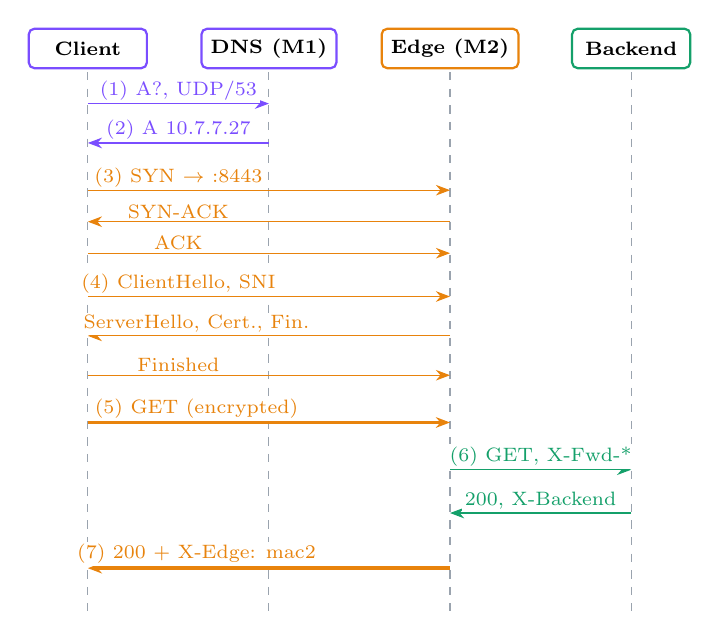
\begin{tikzpicture}[font=\scriptsize, >={Stealth[length=1.8mm]},
  lab/.style={above, fill=white, inner sep=1pt}]
\foreach \x/\n/\c in {0/Client/dns, 2.3/DNS (M1)/dns, 4.6/Edge (M2)/edge, 6.9/Backend/bka}{
  \node[draw=\c, thick, rounded corners=2pt, fill=white, minimum width=1.5cm, minimum height=0.5cm] at (\x,0) {\textbf{\n}};
  \draw[rule, dashed] (\x,-0.3) -- (\x,-7.15);
}
\draw[->, dns]  (0,-0.7) -- node[lab]{(1) A?, UDP/53} (2.3,-0.7);
\draw[->, dns]  (2.3,-1.2) -- node[lab]{(2) A 10.7.7.27} (0,-1.2);
\draw[->, edge] (0,-1.8) -- node[lab, pos=0.25]{(3) SYN $\rightarrow$ :8443} (4.6,-1.8);
\draw[->, edge] (4.6,-2.2) -- node[lab, pos=0.75]{SYN-ACK} (0,-2.2);
\draw[->, edge] (0,-2.6) -- node[lab, pos=0.25]{ACK} (4.6,-2.6);
\draw[->, edge] (0,-3.15) -- node[lab, pos=0.25]{(4) ClientHello, SNI} (4.6,-3.15);
\draw[->, edge] (4.6,-3.65) -- node[lab, pos=0.7]{ServerHello, Cert., Fin.} (0,-3.65);
\draw[->, edge] (0,-4.15) -- node[lab, pos=0.25]{Finished} (4.6,-4.15);
\draw[->, edge, very thick] (0,-4.75) -- node[lab, pos=0.3]{(5) GET (encrypted)} (4.6,-4.75);
\draw[->, bka] (4.6,-5.35) -- node[lab]{(6) GET, X-Fwd-*} (6.9,-5.35);
\draw[->, bka] (6.9,-5.9) -- node[lab]{200, X-Backend} (4.6,-5.9);
\draw[->, edge, very thick] (4.6,-6.6) -- node[lab, pos=0.7]{(7) 200 + X-Edge: mac2} (0,-6.6);
\end{tikzpicture}
\caption{Message sequence for one request. The client validates the certificate between steps
(4) and (5); everything from step (5) onwards is encrypted on the wire up to the edge.}
\label{fig:seq}
\end{figure}

\begin{table}[t]
\caption{Protocol-to-Layer Mapping}
\label{tab:layers}
\centering\footnotesize
\begin{tabularx}{\columnwidth}{@{}P{1.6cm}P{1.25cm}L@{}}
\toprule
\textbf{OSI} & \textbf{TCP/IP} & \textbf{In this project}\\
\midrule
7 Application & Application & DNS, HTTP/1.1, HTTP/2 (standby edge), REST/JSON\\
6 Presentation & Application & TLS encryption, X.509 certificate encoding\\
5 Session & Application & TLS session establishment and resumption\\
4 Transport & Transport & TCP 8443, 8080, 3001, 3002; UDP 53\\
3 Network & Internet & IPv4 /19 addressing, ICMP ping, \code{pf} filtering\\
2 Data link & Link & Wi-Fi frames, MAC addresses, ARP\\
1 Physical & Link & IEEE 802.11 radio\\
\bottomrule
\end{tabularx}
\end{table}

\subsection{Configuration Management}
A single file, \code{team.env}, holds the team name, the four addresses, the backup DNS and
standby edge addresses and the port numbers. A helper script (\code{setup\_team.sh}) rewrites it,
rejecting malformed addresses and the gateway address, and \code{sync.sh} copies it together with
the shared scripts into one folder per laptop. Every script refuses to run if the address in
\code{team.env} does not belong to the host it is run on. This guard proved its value when the
campus DHCP service reassigned all four addresses during the project: the scripts stopped with an
explicit message instead of failing silently, the file was updated once and redistributed through
the team's Git repository, and work resumed.

% =====================================================================
\section{Phase 1: Build and Observe}
\label{sec:p1}

Table~\ref{tab:p1} summarises the seven mandatory tasks. The status column distinguishes evidence
captured during the lab session (\emph{Verified}), evidence captured afterwards with the same code
and configuration (\emph{Reproduced}) and items supported only by indirect evidence
(\emph{Explained}).

\begin{table}[t]
\caption{Phase 1 Task Summary}
\label{tab:p1}
\centering\footnotesize
\begin{tabularx}{\columnwidth}{@{}P{0.45cm}LP{1.35cm}@{}}
\toprule
\textbf{Task} & \textbf{Success condition and observed result} & \textbf{Status}\\
\midrule
A & All four hosts on one subnet; full ping matrix succeeds & Verified\\
B & Two or more clients resolve \code{app.team1.test} to 10.7.7.27 via Mac 1 (three clients) & Verified\\
C & Both backends reachable from another host; distinct \code{X-Backend} & Verified\\
D & Round-robin A, B, A, B through the edge & Verified\\
E & HTTPS by name, no \code{-k}; \code{Verify return code: 0 (ok)}; TLS 1.3 & Verified\\
F & \code{Cache-Control}, \code{ETag}, \code{304 Not Modified} & Reproduced\\
G & DNS, TCP, TLS and encrypted data identified per layer & Explained\\
\bottomrule
\end{tabularx}
\end{table}

\subsection{Task A: Private LAN}
Each member ran \code{my\_ip.sh}, which prints the interface, IPv4 address, netmask, gateway, DHCP
server, MAC address and active DNS resolvers, and then pings the gateway. \code{check\_lan.sh}
pings every team host; the matrix captured from Mac~2 reported \code{OK} for all four addresses
(Mac~2: \code{en0}, MAC \code{9e:ed:71:95:bb:39}). The first run on Mac~1 printed a warning that
the active resolver was \code{127.0.2.2}, the local proxy of a VPN client, which would have
bypassed the team DNS server; the client was disabled before continuing.

\subsection{Task B: Private DNS Server}
\code{setup\_dnsmasq.sh primary} installs dnsmasq~\cite{dnsmasq}, generates the configuration in
Listing~\ref{lst:dnsmasq} (Appendix~\ref{app:config}), validates it with \code{dnsmasq -{}-test}
and restarts the service. The \code{local=/team1.test/} directive makes the server authoritative
for the team zone so that those names are never forwarded; all other names are forwarded to
public resolvers so the clients keep Internet access. The self-test (Listing~\ref{lst:selftest};
screenshot in Fig.~\ref{fig:dnsmasq}) shows dnsmasq bound to \code{10.7.9.43:53} and
\code{127.0.0.1:53} and answering with the edge address. A query issued from Mac~2 to Mac~1
returned the same record, confirming that the server answers other hosts.
\begin{lstlisting}[caption={Primary DNS self-test on Mac 1 (dnsmasq 2.93)},label={lst:selftest}]
dnsmasq: syntax check OK.
dnsmasq 69690 nobody  4u  IPv4  UDP 10.7.9.43:53
dnsmasq 69690 nobody  6u  IPv4  UDP 127.0.0.1:53
$ dig app.team1.test @10.7.9.43 +noall +answer
app.team1.test.     0    IN    A    10.7.7.27
\end{lstlisting}

Clients were switched with \code{set\_dns.sh primary}, which first saves the existing resolver
setting so that it can be restored, then sets the resolver and flushes the system cache. Three
clients (Mac~1, Mac~3, Mac~4) resolved through the team server, exceeding the requirement of two.

\subsection{Task C: REST Backends}
Both backends run the same Flask~\cite{flask} application (excerpt in
Listing~\ref{lst:backend}); only an environment file differs (\code{BACKEND\_ID=A}, port 3001 on
Mac~3; \code{B}, port 3002 on Mac~4). The application binds to \code{0.0.0.0}; binding to the
loopback address would make it unreachable from the edge and produce a 502. Every response
carries \code{X-Backend} and \code{X-Response-Time-ms}. The endpoints are \code{/api/status}
(dynamic, \code{no-store}), \code{/api/catalog} (cacheable, with ETag), \code{/api/whoami}
(echoes the peer and the forwarded client headers) and \code{/health} (uptime and request
counter). Each request is also logged with the peer address and whether it arrived \emph{via
edge} or \emph{direct}. From Mac~1, both backends answered directly with HTTP~200 and their own
identifier, and \code{nc} confirmed that TCP port 3001 was reachable across the LAN.

\subsection{Task D: Reverse Proxy and Load Balancer}
\code{configure\_nginx.sh} renders the nginx configuration from a template using the values in
\code{team.env}, validates it with \code{nginx -t}, and starts or reloads nginx
(Listing~\ref{lst:nginx}). The upstream pool lists both backends with
\code{max\_fails=2 fail\_timeout=10s}; the default round-robin strategy is used, with
\code{least\_conn} noted as an alternative. Port 8080 redirects to HTTPS with a 301. A custom log
format records the selected upstream, the backend identifier and the request time.

Listing~\ref{lst:lb} (screenshot in Fig.~\ref{fig:lb}) shows six consecutive HTTPS requests from
Mac~1, validated without bypass flags. Responses alternate A, B, A, B, A, B, each with status~200
and \code{X-Edge: mac2}. The edge access log independently records the same alternation:
\begin{lstlisting}[caption={Load-balancing gate from Mac 1 (demo\_lb.sh)},label={lst:lb}]
GET https://app.team1.test:8443/api/status x6 (no -k)
 1  HTTP/1.1 200 OK   X-Backend: A   X-Edge: mac2
 2  HTTP/1.1 200 OK   X-Backend: B   X-Edge: mac2
 3  HTTP/1.1 200 OK   X-Backend: A   X-Edge: mac2
 4  HTTP/1.1 200 OK   X-Backend: B   X-Edge: mac2
 5  HTTP/1.1 200 OK   X-Backend: A   X-Edge: mac2
 6  HTTP/1.1 200 OK   X-Backend: B   X-Edge: mac2
\end{lstlisting}
\begin{lstlisting}[caption={Edge access log on Mac 2 (custom format)},label={lst:access}]
10.7.9.43 "GET /api/status HTTP/1.1" 200 backend=10.7.29.229:3001 xb=A rt=0.046
10.7.9.43 "GET /api/status HTTP/1.1" 200 backend=10.7.25.176:3002 xb=B rt=0.157
\end{lstlisting}

\subsection{Task E: HTTPS and TLS}
Because public CAs do not issue certificates for reserved names, the team operated its own CA
(\emph{team1 Local CA}). \code{make\_certs.sh} on Mac~2 generates a 4096-bit RSA CA key and a
self-signed CA certificate (\code{CA:TRUE}, 825 days), then a 2048-bit server key and a
certificate signing request, and signs the server certificate with SHA-256 for 365 days with
\code{subjectAltName = DNS:app.team1.test, DNS:api.team1.test} and
\code{extendedKeyUsage = serverAuth}. Because the certificate contains names rather than
addresses, it remained valid after the DHCP reassignment and could be reused unchanged by the
standby edge in Phase~2.

Only the public CA certificate was distributed: \code{serve\_ca.sh} served it on port 8000 from a
directory that contains no private keys, and the server log (Fig.~\ref{fig:ca}) records one
download by each of the three other members. On each client, \code{trust\_ca.sh} printed the
certificate fingerprint and added the CA to the macOS System keychain; all three clients printed
the same SHA-256 fingerprint (\code{62:F0:8C:C0:78:C5:16:67:\ldots:2B:31:D9}). Private keys were
never committed to the repository.

Listing~\ref{lst:tls} summarises the TLS verification run from Mac~1 (full output in
Fig.~\ref{fig:tls}). The handshake negotiated
TLS~1.3 (\code{TLS\_AES\_256\_GCM\_SHA384} via OpenSSL), the subject was
\code{CN=app.team1.test}, the issuer \code{CN=team1 Local CA}, and both curl
(\code{SSL certificate verify ok}) and OpenSSL (\code{Verify return code: 0 (ok)}) accepted the
chain. Forcing TLS~1.2 exposes the full message sequence (Certificate, ServerKeyExchange,
ServerHelloDone, ClientKeyExchange, ChangeCipherSpec, Finished), which is the variant used for
packet inspection because the certificate is visible on the wire.
\begin{lstlisting}[float=tb,caption={TLS verification from Mac 1 (demo\_tls.sh, excerpt)},label={lst:tls}]
* Connected to app.team1.test (10.7.7.27) port 8443
* SSL connection using TLSv1.3 / AEAD-CHACHA20-POLY1305-SHA256
*  subject: CN=app.team1.test
*  issuer: CN=team1 Local CA
*  SSL certificate verify ok.
< HTTP/1.1 200 OK
-- openssl s_client --
New, TLSv1.3, Cipher is TLS_AES_256_GCM_SHA384
Verify return code: 0 (ok)
-- forced TLS 1.2 --
* TLSv1.2 (IN), TLS handshake, Certificate (11)
* TLSv1.2 (IN), TLS handshake, Server key exchange (12)
* TLSv1.2 (IN), TLS handshake, Server finished (14)
* TLSv1.2 (OUT), TLS handshake, Client key exchange (16)
* TLSv1.2 (OUT), TLS change cipher, Change cipher spec (1)
* TLSv1.2 (OUT), TLS handshake, Finished (20)
* SSL connection using TLSv1.2 / ECDHE-RSA-CHACHA20-POLY1305
\end{lstlisting}

The primary edge's nginx build lacked the HTTP/2 module and therefore served HTTP/1.1, which the
brief permits; the standby edge in Phase~2 answered over HTTP/2.

\subsection{Task F: HTTP Caching}
\code{/api/catalog} returns \code{Cache-Control: max-age=60} and an ETag derived from a SHA-256
hash of the body. Because both backends return an identical body, they compute an identical
ETag, so revalidation succeeds regardless of which backend answers. The test sequence was:
\begin{lstlisting}
GET /api/catalog                -> 200 OK, ETag: "0ee15ab3a9bc1a9c", Cache-Control: max-age=60
GET /api/catalog
  If-None-Match: "0ee15ab3a9bc1a9c" -> 304 NOT MODIFIED (no body)
HEAD /api/status                -> 200 OK, Cache-Control: no-store
\end{lstlisting}
Within the 60~s freshness window a browser reuses the response with no request at all (a fresh
cache hit); after it, the client sends a conditional request and receives a body-less 304 (a
validated hit); a hard reload bypasses the cache and returns a full 200 (a new request). This
sequence was reproduced on Mac~2 after the lab session against the same \code{backend.py},
because the lab backends had been stopped by then; nginx forwards these headers unchanged.

\subsection{Task G: Protocol Flow}
Table~\ref{tab:wire} lists, for each phase of a request, the Wireshark~\cite{wireshark} display
filter used to isolate it, the expected observation and the evidence that corroborates it. The
capture file itself was not retained (see Section~\ref{sec:limits}); the TLS message sequence in
Listing~\ref{lst:tls}, the DNS answers and the TCP connection checks are the supporting evidence.

\begin{table}[t]
\caption{Protocol Flow: Filters, Observations and Evidence}
\label{tab:wire}
\centering\footnotesize
\begin{tabularx}{\columnwidth}{@{}P{2.25cm}LP{1.3cm}@{}}
\toprule
\textbf{Filter} & \textbf{Expected observation} & \textbf{Evidence}\\
\midrule
\code{dns} & Query for app.team1.test from an ephemeral port to UDP/53; answer 10.7.7.27 with TTL & Listing~\ref{lst:selftest}\\
\code{tcp.flags.syn==1}\newline\code{\&\& tcp.port==8443} & SYN, SYN-ACK, ACK between an ephemeral client port and 8443 & \code{nc} to 8443 succeeded\\
\code{tls.handshake} & ClientHello with SNI, ServerHello, Certificate (TLS 1.2), Finished & Listing~\ref{lst:tls}\\
\code{tls.record.}\newline\code{content\_type==23} & Application Data only; HTTP request and JSON unreadable & Listing~\ref{lst:tls}\\
\bottomrule
\end{tabularx}
\end{table}

\subsection{Explanation-Only Topics}
HTTP/3 replaces TCP with QUIC over UDP, merging the transport and TLS handshakes; it was not
deployed. Content delivery networks apply the same \code{Cache-Control} and validator semantics
shown in Task~F at geographically distributed edges, which corresponds to the edge role of
Mac~2. Email protocols (SMTP, IMAP, POP3) are outside the request path of this platform and were
treated conceptually only.

% =====================================================================
\section{Phase 1: Required Failure Demonstrations}
\label{sec:fail}

Five faults were injected, each confined to one layer (Table~\ref{tab:fail}). The scripted
procedure is \code{failures.sh} with arguments 1 to 5, run on a client.

\begin{table*}[t]
\caption{Failure Demonstrations: Injection, Symptom and First Failing Layer}
\label{tab:fail}
\centering\footnotesize
\begin{tabularx}{\textwidth}{@{}P{0.3cm}P{3.0cm}P{3.6cm}LP{1.55cm}P{1.45cm}@{}}
\toprule
\textbf{\#} & \textbf{Fault} & \textbf{Injection} & \textbf{Observed symptom} & \textbf{Layer} & \textbf{Status}\\
\midrule
1 & Wrong DNS server on the client & Resolver set to unused 10.7.9.250 & \code{dig}: \emph{connection timed out; no servers could be reached}; ping to Mac~1 and TCP connect to 10.7.7.27:8443 still succeed & DNS (service) & Reproduced\\
2 & Record points to a wrong IP & \code{APP\_IP=10.7.25.176} on Mac~1 & Resolution succeeds with no error but returns the wrong host; the connection is refused at that host & DNS (data) & Explained\\
3 & One backend stopped & Stop Backend A & Edge skips the failed upstream and serves from the survivor; access log shows \code{backend=...:3002, ...:3001} on one request & Backend & Explained\\
4 & Both backends stopped & Stop A and B & DNS returns 10.7.7.27; TLS \code{Verify return code: 0}; HTTP \code{502 Bad Gateway} with \code{X-Edge: mac2}; error log: \emph{connect() failed (61: Connection refused)} for both upstreams & Backend (upstream) & Reproduced\\
5 & Wrong destination port & Connect to 9999 & Host reachable; \emph{Connection refused} immediately (TCP RST) & Transport & Reproduced\\
\bottomrule
\end{tabularx}
\end{table*}

The demonstrations separate concerns that are easily conflated. Failure~1 shows that name
resolution and IP reachability are independent: the hosts remain reachable by address while
lookup fails. Failure~2 shows that DNS is a directory rather than a connection, so a successful
lookup does not guarantee a correct destination; this is why the diagnostic script checks the
returned address and not only the response code. Failure~4 locates the boundary between edge and
backend: every layer up to TLS succeeds, and the 502 is generated by nginx itself. Failure~5
contrasts an immediate refusal (a reset from a reachable host) with the timeout produced by a
silent drop in Phase~2.

% =====================================================================
\section{Phase 2: Harden, Recover and Troubleshoot}
\label{sec:p2}

Each member executed a role-specific runner (\code{phase2.sh}) that sequenced the steps, paused
at synchronisation points between hosts and saved terminal output and screenshots as evidence.

\subsection{Extension A: Backup DNS Resolver}
A second dnsmasq instance on Mac~3 (\code{setup\_dnsmasq.sh backup}) serves the same zone. Both
servers returned \code{10.7.7.27}. Mac~1 was configured with both resolvers in order
(\code{set\_dns.sh both}), and the primary service was stopped. A query to the primary timed
out, the backup still answered, and a full HTTPS request by name completed with status~200 in
2.552~s. The additional latency is the resolver's timeout on the first server before it moves to
the second, so resolver-list failover preserves availability at the cost of one timeout.

\subsection{Extension B: TTL and Controlled Record Change}
Both servers were restarted with \code{host-record} entries carrying a 30~s TTL. While
\code{demo\_ttl.sh} sampled every 5~s both a direct query to Mac~1 (always fresh) and the system
resolver (cached), the record was changed to \code{10.7.25.176}. Fig.~\ref{fig:ttl} shows the
result: the authoritative answer changed at 11:05:51, whereas the system resolver continued to
return the old address until 11:06:22 and switched at 11:06:27, immediately after a scheduled
cache flush. The stale answer therefore survived the change for more than 30~s. Because the
switch coincided with the flush, natural expiry and the flush cannot be separated in this run.
The practical implication is that a planned migration should lower the TTL well before the
change.

\begin{figure}[t]
\centering
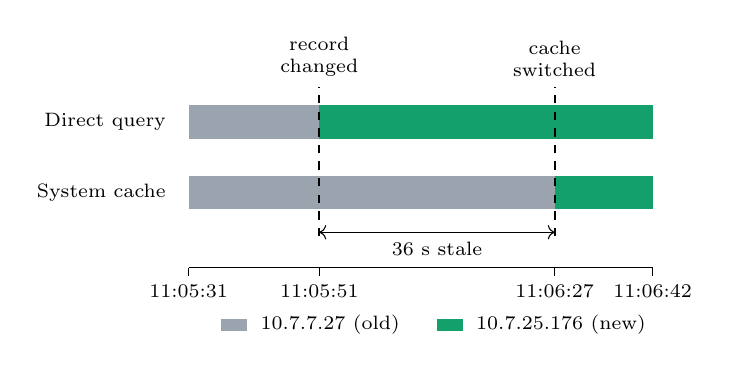
\begin{tikzpicture}[font=\scriptsize, x=0.083cm]
\def\h{0.42}
\node[anchor=east] at (-2,0.9) {Direct query};
\node[anchor=east] at (-2,0) {System cache};
\fill[old] (0,0.9-\h/2) rectangle (20,0.9+\h/2);
\fill[new] (20,0.9-\h/2) rectangle (71,0.9+\h/2);
\fill[old] (0,-\h/2) rectangle (56,\h/2);
\fill[new] (56,-\h/2) rectangle (71,\h/2);
\draw[dashed, thick] (20,-0.55) -- (20,1.35) node[above, align=center] {record\\changed};
\draw[dashed, thick] (56,-0.55) -- (56,1.35) node[above, align=center] {cache\\switched};
\draw[<->] (20,-0.5) -- node[below] {36 s stale} (56,-0.5);
\draw (0,-0.95) -- (71,-0.95);
\foreach \t/\l in {0/11:05:31, 20/11:05:51, 56/11:06:27, 71/11:06:42}
  {\draw (\t,-0.95) -- (\t,-1.05) node[below] {\l};}
\fill[old] (5,-1.75) rectangle (9,-1.6); \node[anchor=west] at (9.5,-1.675) {10.7.7.27 (old)};
\fill[new] (38,-1.75) rectangle (42,-1.6); \node[anchor=west] at (42.5,-1.675) {10.7.25.176 (new)};
\end{tikzpicture}
\caption{TTL experiment (TTL = 30~s, 5~s sampling). The cached answer outlived the record change
by 36~s; the switch followed a cache flush.}
\label{fig:ttl}
\end{figure}

\subsection{Extension C: Service Isolation}
\code{isolate\_pf.sh} on each backend saves a rollback copy of \code{/etc/pf.conf} and the active
rule set, appends two rules and enables \code{pf} (Listing~\ref{lst:pf}): TCP to the backend port
is passed only from the edge (10.7.7.27) and silently dropped from every other source. The rules
were confirmed active on both Mac~3 (port 3001) and Mac~4 (port 3002), and
\code{rollback\_pf.sh} restored both hosts, reporting \emph{rules identical to before}. With the
rules active, a client connecting directly to a backend port should time out while requests
through the edge continue to succeed. This is least-privilege access, equivalent to a cloud
security group that admits only the load balancer. The two connectivity checks intended to show
this were not captured at the right moment (Section~\ref{sec:limits}). Source-address rules can be
spoofed on a shared segment, so this demonstrates the principle rather than a hardened control.

\subsection{Extension D: High-Availability Failover}
nginx uses passive health checks: after two failed attempts (\code{max\_fails=2}) a server is
skipped for \code{fail\_timeout=10s}, and a failed request is retried on the next server
(\code{proxy\_next\_upstream error timeout http\_502 http\_503 http\_504}, two tries) with a 2~s
connect timeout. The access log contains two requests that demonstrate this behaviour directly:
\begin{lstlisting}
"HEAD /api/status" 200 backend=10.7.25.176:3002, 10.7.29.229:3001 xb=A rt=2.123
"HEAD /api/status" 200 backend=10.7.25.176:3002, 10.7.29.229:3001 xb=A rt=1.029
\end{lstlisting}
In each case nginx first selected Backend~B, the attempt failed within the connect timeout, and
the request was transparently served by Backend~A; the client received status~200. The planned
stop-and-restart of Backend~A did not take effect because the stop command matched the process
name case-sensitively (Section~\ref{sec:disc}); the script was corrected to stop the process
listening on the port.

\subsection{Extension E: Controlled Edge Migration}
The single edge is the remaining single point of failure. A standby edge was built on Mac~3:
Mac~2 transferred the server certificate and key to Mac~3 only (\code{serve\_certs.sh}), and
\code{configure\_nginx.sh standby} started nginx with the same upstream pool and the header
\code{X-Edge: standby}. Queried directly, the standby answered \code{HTTP/2 200} with
\code{x-backend: A} and was listening on \code{*:8443}.

While \code{demo\_edge.sh} sampled the serving edge every 5~s, the DNS record (TTL 30~s) was
changed from 10.7.7.27 to 10.7.29.229 at approximately 11:07:51. Fig.~\ref{fig:cut} shows that
traffic was served by Mac~2 until 11:08:07, one sample at 11:08:14 was indeterminate while the
resolver switched, and from 11:08:19 every request was served by the standby with the backends
still alternating. The cutover took approximately 28~s, consistent with the 30~s TTL. The same
certificate was valid on the standby because it binds names, not addresses.

\begin{figure}[t]
\centering
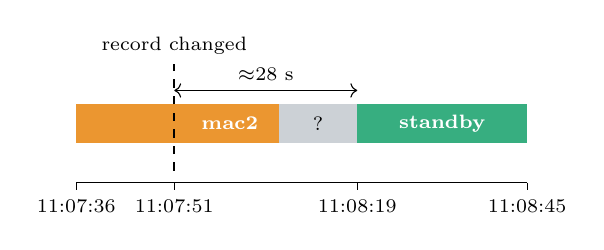
\begin{tikzpicture}[font=\scriptsize, x=0.083cm]
\def\h{0.5}
\fill[edge!85] (0,-\h/2) rectangle (31,\h/2);
\fill[rule!50] (31,-\h/2) rectangle (43,\h/2);
\fill[bka!85] (43,-\h/2) rectangle (69,\h/2);
\node[white, font=\scriptsize\bfseries] at (23.5,0) {mac2};
\node at (37,0) {?};
\node[white, font=\scriptsize\bfseries] at (56,0) {standby};
\draw[dashed, thick] (15,-0.6) -- (15,0.75) node[above] {record changed};
\draw[<->] (15,0.42) -- node[above] {$\approx$28 s} (43,0.42);
\draw (0,-0.75) -- (69,-0.75);
\foreach \t/\l in {0/11:07:36, 15/11:07:51, 43/11:08:19, 69/11:08:45}
  {\draw (\t,-0.75) -- (\t,-0.85) node[below] {\l};}
\end{tikzpicture}
\caption{DNS-based edge cutover from Mac~2 to the standby edge on Mac~3 (TTL = 30~s, 5~s
sampling). Backends continued to alternate A/B behind both edges.}
\label{fig:cut}
\end{figure}

\subsection{Extension F: Troubleshooting Methodology}
\code{diagnose.sh} checks the stack bottom-up and stops the reader at the first failure:
(0)~gateway and edge reachability; (1)~DNS response code, returned address and agreement of the
system resolver; (2)~TCP connect to the edge port; (3)~certificate verification; (4)~HTTP status
through the edge; and (5)~direct backend health. Each failure prints its most likely causes.
Table~\ref{tab:diag} lists the mapping used during the challenge. A healthy run passed every
layer (Fig.~\ref{fig:diagpair}(b)), and the final readiness check (\code{phase2\_check.sh}) reported
\emph{ready: 9, not ready: 0}, covering both resolvers, the edge, both backends and both edge
identities.

The method was validated in practice during Phase~1. The first diagnostic run
(Listing~\ref{lst:falsefail}; Fig.~\ref{fig:diagpair}(a)) reported a failure at the TLS layer
(\code{Verify return code: 21}) while the HTTP check immediately above it returned 200 without
bypass flags. A genuine TLS failure would have prevented the HTTPS request, so the inconsistency
pointed to the test rather than the system: the OpenSSL build shipped with macOS (LibreSSL) does
not consult the system keychain in which the CA had been installed, whereas curl does. Passing the
CA file explicitly (\code{-CAfile}) corrected the check, after which every layer passed.
\begin{lstlisting}[caption={First diagnostic run (excerpt): inconsistent layers},label={lst:falsefail}]
== 2. TCP layer ==
PASS  edge port 8443 open
== 3. TLS layer ==
Verify return code: 21 (unable to verify the first certificate)
FAIL  expired cert / SAN mismatch / CA not trusted / wrong cert-key pair
== 4. HTTP / application layer (through the edge) ==
HTTP status: 200
PASS  200 via edge
\end{lstlisting}

\begin{table}[t]
\caption{First Failing Layer, Likely Cause and Remedy}
\label{tab:diag}
\centering\footnotesize
\begin{tabularx}{\columnwidth}{@{}P{1.55cm}LP{2.3cm}@{}}
\toprule
\textbf{First FAIL} & \textbf{Likely cause} & \textbf{Remedy}\\
\midrule
IP/LAN & Different network, VPN, client isolation & Rejoin network; disable VPN\\
DNS (no answer) & dnsmasq stopped; wrong client resolver & Restart dnsmasq; \code{set\_dns.sh primary}\\
DNS (wrong IP) & Wrong record; stale cache & Fix record; flush cache\\
TCP & nginx stopped; wrong port; filter & Start nginx; check port\\
TLS & CA not trusted; SAN mismatch; expiry & \code{trust\_ca.sh}; reissue\\
HTTP 502/504 & Backends down; wrong upstream & Start backends; fix upstream\\
Backends (direct) & Stopped; bound to 127.0.0.1; \code{pf} & Bind 0.0.0.0; \code{rollback\_pf.sh}\\
\bottomrule
\end{tabularx}
\end{table}

% =====================================================================
\section{Phase 2 Final Report}
\label{sec:p2report}

\subsection{What Changed from Phase 1}
Table~\ref{tab:changes} summarises the architectural changes.

\begin{table}[t]
\caption{Changes from Phase 1 to Phase 2}
\label{tab:changes}
\centering\footnotesize
\begin{tabularx}{\columnwidth}{@{}P{1.3cm}P{2.3cm}L@{}}
\toprule
\textbf{Area} & \textbf{Phase 1} & \textbf{Phase 2}\\
\midrule
DNS & Single dnsmasq on Mac 1 & Backup dnsmasq on Mac 3; clients list both\\
TTL & 0 s (no caching) & 30 s \code{host-record} for experiments\\
Backends & Reachable by any LAN host & \code{pf}: only the edge may connect\\
Failover & Configured, not exercised & Passive checks and retries demonstrated\\
Edge & Single nginx on Mac 2 & Standby nginx on Mac 3; DNS cutover\\
Diagnosis & Ad hoc & Scripted bottom-up procedure\\
\bottomrule
\end{tabularx}
\end{table}

\subsection{Resilience Test Results}
Table~\ref{tab:results} reports the outcome of each extension.

\begin{table*}[t]
\caption{Phase 2 Resilience Test Results}
\label{tab:results}
\centering\footnotesize
\begin{tabularx}{\textwidth}{@{}P{2.6cm}P{4.0cm}LP{2.4cm}@{}}
\toprule
\textbf{Extension} & \textbf{Test} & \textbf{Observation} & \textbf{Status}\\
\midrule
A. Backup DNS & Stop primary dnsmasq; resolve and fetch by name & Primary timed out; backup answered 10.7.7.27; HTTPS 200 in 2.552 s & Verified\\
B. TTL & Change record under TTL = 30 s & Authoritative change 11:05:51; cache stale until 11:06:22 (36 s); switched after flush & Verified\\
C. Isolation & \code{pf} pass from edge, drop others; rollback & Rules active on both backends; rollback identical; block not captured live & Verified with notes\\
D. HA failover & Upstream failure during requests & Requests retried on the other backend (rt 2.123 s, 1.029 s), client got 200; planned stop did not occur & Verified with notes\\
E. Edge migration & Repoint DNS to standby edge & \code{X-Edge} mac2 $\rightarrow$ standby in $\approx$28 s; backends kept alternating & Verified\\
F. Troubleshooting & Inject fault; diagnose bottom-up & Healthy and final runs all PASS (9/9 ready); fault run captured before injection & Verified with notes\\
\bottomrule
\end{tabularx}
\end{table*}

\subsection{Troubleshooting Findings}
Three findings generalise beyond this project. First, reading the layers in order exposes
inconsistent results: a failure at a lower layer combined with success at a higher one indicates a
faulty test, as with the LibreSSL keychain issue. Second, the symptom identifies the layer:
a DNS timeout points to the resolver, an immediate refusal to a closed port on a reachable host, a
connect timeout to filtering or an absent host, and a 502 after a valid TLS handshake to the
backends. Third, host-level controls interfere with network tests: a macOS \emph{Local Network}
privacy prompt blocked a terminal's LAN traffic and produced a refusal within 2~ms that resembled a
network fault.

\subsection{Learning Summary}
\emph{Extension A.} Resolver redundancy keeps names resolvable when a server fails, but clients try
servers in order and pay one timeout before falling back; availability is preserved while latency
rises.

\emph{Extension B.} TTL is the price of caching. After a record changes, clients may use the old
answer for up to one TTL, so migrations should be prepared by lowering the TTL in advance, and the
system cache must be considered separately from what the authoritative server returns.

\emph{Extension C.} Restricting backend ports to the edge enforces least privilege and prevents
clients from bypassing TLS and load balancing. A silent drop produces a timeout rather than a
refusal, and a rollback copy is essential when modifying host firewalls.

\emph{Extension D.} Passive health checks detect failures through real traffic; combined with
request retries they hide a failed backend from clients at the cost of one connect timeout on the
affected request.

\emph{Extension E.} DNS-based cutover removes the edge as a single point of failure, but it is
manual and bounded by the TTL; automatic failover would require a virtual IP protocol such as VRRP
(e.g., keepalived) or a managed load balancer. Name-based certificates make the standby
interchangeable with the primary.

\emph{Extension F.} A fixed bottom-up order turns troubleshooting into a procedure: the first
failing layer is the cause, and the layers above it fail as consequences.

% =====================================================================
\section{Discussion}
\label{sec:disc}

\subsection{Mapping to Cloud Services}
The platform reproduces a common cloud pattern at small scale: dnsmasq plays the role of a
managed DNS service such as Route~53 (including failover records in Extension~A and E), nginx the
role of an application load balancer or CDN edge with TLS termination, the backends the role of
compute instances, and \code{pf} the role of security groups.

\subsection{Remaining Single Point of Failure}
After Phase~2, DNS and backends are redundant, but switching edges still requires a manual record
change and up to one TTL of delay. A floating virtual IP shared by the two edges would make the
switch automatic and independent of client caches.

\subsection{Problems Encountered}
Table~\ref{tab:issues} records the practical problems met during the work and their resolution.

\begin{table}[t]
\caption{Problems Encountered and Resolutions}
\label{tab:issues}
\centering\footnotesize
\begin{tabularx}{\columnwidth}{@{}P{2.3cm}L@{}}
\toprule
\textbf{Problem} & \textbf{Cause and resolution}\\
\midrule
All IPs changed & Campus DHCP renewal; scripts refused to run. \code{team.env} updated once and redistributed; certificates unaffected.\\
Team DNS ignored & VPN client resolver at 127.0.2.2; detected by a warning, client disabled.\\
False TLS failure & LibreSSL ignores the keychain; CA file passed with \code{-CAfile}.\\
Backend would not stop & Process matched as \code{python}, macOS reports \code{Python}; now stopped by port.\\
LAN blocked from terminal & macOS Local Network permission; granted in Privacy settings.\\
Steps out of order & Tests ran before the fault or filter was in place; scripts now warn when the precondition is missing.\\
\bottomrule
\end{tabularx}
\end{table}

% =====================================================================
\section{Limitations}
\label{sec:limits}
The following limitations qualify the results and are stated so that each claim can be weighed
against its evidence.
\begin{itemize}
\item \emph{Packet capture.} A Wireshark capture file was not retained. Task~G is supported by
the TLS message sequence, DNS answers and TCP connection checks rather than by a capture.
\item \emph{Post-lab reproduction.} The caching test and failures~1, 4 and~5 were captured on
Mac~2 after the lab session with the same code and configuration, because the lab backends had
been stopped. Failures~2 and~3 are supported by the TTL experiment and the failover log lines
rather than by dedicated captures.
\item \emph{Extension C.} The rules and their rollback are evidenced on both backends, but the
client-side check ran before the rules were enabled (it still returned 200) and the edge-side
check was blocked by the macOS Local Network prompt, so the block itself was not captured.
\item \emph{Extension D.} The planned stop of Backend~A did not take effect; failover is evidenced
by the two retried requests in the edge access log.
\item \emph{Extension F.} The fault run was captured before nginx was stopped; the edge-side log
confirms that the fault was injected afterwards.
\item \emph{Measurement resolution.} Timelines were sampled every 5~s, so the reported cutover
and staleness durations are accurate to about one sampling interval.
\end{itemize}

% =====================================================================
\section{Conclusion}
The team built a complete private service platform from naming to application on four laptops and
verified every layer of a request with independent evidence: private DNS answered three clients,
TLS~1.3 was validated against a team CA without bypass flags, the edge alternated requests between
two backends, and caching produced conditional 304 responses. Five controlled failures were each
confined to a single layer. Phase~2 added a backup resolver that preserved availability with a
2.55~s penalty, quantified a 36~s stale-cache window under a 30~s TTL, isolated the backend ports
behind the edge, demonstrated transparent retry on upstream failure, and migrated traffic to a
standby edge in approximately 28~s. The remaining single point of failure is the manual edge
switch, which a virtual-IP failover protocol would remove. The limitations listed above identify
the items whose live evidence should be repeated: a packet capture, the isolation block, a clean
backend stop and an injected-fault diagnosis.

\section*{Acknowledgment}
The authors thank the faculty of the Computer Networks course at Rishihood University for the
project brief and guidance.

% =====================================================================
\begin{thebibliography}{99}
\bibitem{brief} Rishihood University, ``Computer Networks course project: Private network service
platform, a two-phase, team-based local networking project,'' Project brief, 2026.
\bibitem{rfc1034} P.~Mockapetris, ``Domain names: Concepts and facilities,'' RFC 1034, IETF, 1987.
\bibitem{rfc1035} P.~Mockapetris, ``Domain names: Implementation and specification,'' RFC 1035,
IETF, 1987.
\bibitem{rfc2606} D.~Eastlake 3rd and A.~Panitz, ``Reserved top level DNS names,'' RFC 2606, IETF,
1999.
\bibitem{rfc6762} S.~Cheshire and M.~Krochmal, ``Multicast DNS,'' RFC 6762, IETF, 2013.
\bibitem{rfc9293} W.~Eddy, Ed., ``Transmission Control Protocol (TCP),'' RFC 9293, IETF, 2022.
\bibitem{rfc8446} E.~Rescorla, ``The Transport Layer Security (TLS) protocol version 1.3,''
RFC 8446, IETF, 2018.
\bibitem{rfc5246} T.~Dierks and E.~Rescorla, ``The Transport Layer Security (TLS) protocol version
1.2,'' RFC 5246, IETF, 2008.
\bibitem{rfc5280} D.~Cooper \emph{et al.}, ``Internet X.509 public key infrastructure certificate
and certificate revocation list (CRL) profile,'' RFC 5280, IETF, 2008.
\bibitem{rfc9110} R.~Fielding, M.~Nottingham, and J.~Reschke, Eds., ``HTTP semantics,'' RFC 9110,
IETF, 2022.
\bibitem{rfc9111} R.~Fielding, M.~Nottingham, and J.~Reschke, Eds., ``HTTP caching,'' RFC 9111,
IETF, 2022.
\bibitem{nginxup} NGINX, ``Module ngx\_http\_upstream\_module,'' [Online]. Available:
\url{https://nginx.org/en/docs/http/ngx_http_upstream_module.html}
\bibitem{nginxproxy} NGINX, ``Module ngx\_http\_proxy\_module,'' [Online]. Available:
\url{https://nginx.org/en/docs/http/ngx_http_proxy_module.html}
\bibitem{dnsmasq} S.~Kelley, ``dnsmasq,'' [Online]. Available:
\url{https://thekelleys.org.uk/dnsmasq/doc.html}
\bibitem{flask} Pallets Projects, ``Flask documentation,'' [Online]. Available:
\url{https://flask.palletsprojects.com/}
\bibitem{pf} OpenBSD, ``pf.conf: packet filter configuration file,'' manual page, [Online].
Available: \url{https://man.openbsd.org/pf.conf}
\bibitem{wireshark} Wireshark Foundation, ``Wireshark user's guide,'' [Online]. Available:
\url{https://www.wireshark.org/docs/}
\bibitem{kurose} J.~F. Kurose and K.~W. Ross, \emph{Computer Networking: A Top-Down Approach},
8th~ed. Hoboken, NJ, USA: Pearson, 2021.
\end{thebibliography}

% =====================================================================
\appendices

\section{Configuration Bundle}
\label{app:config}

\subsection{Primary DNS (Mac 1)}
The backup on Mac~3 differs only in \code{listen-address}. For Extensions~B and~E the
\code{address=} lines are replaced by \code{host-record=<name>,<ip>,30}.
\begin{lstlisting}[caption={dnsmasq.conf generated on Mac 1},label={lst:dnsmasq}]
port=53
listen-address=10.7.9.43,127.0.0.1
bind-interfaces
local=/team1.test/
server=8.8.8.8
server=1.1.1.1
address=/app.team1.test/10.7.7.27
address=/api.team1.test/10.7.7.27
log-queries
log-facility=/tmp/dnsmasq.log
\end{lstlisting}

\subsection{Edge (Mac 2)}
Rendered from \code{nginx.conf.template}; the standby differs only in \code{X-Edge}. The Phase~2
directives (passive checks, retries, \code{X-Edge}) were present from the start.
\begin{lstlisting}[caption={nginx configuration (essential parts)},label={lst:nginx}]
log_format cn '$remote_addr [$time_local] "$request" $status '
              'backend=$upstream_addr xb=$upstream_http_x_backend rt=$request_time';
upstream backends {
  # least_conn;   # alternative to the default round-robin
  server 10.7.29.229:3001 max_fails=2 fail_timeout=10s;   # Backend A
  server 10.7.25.176:3002 max_fails=2 fail_timeout=10s;   # Backend B
}
server {
  listen 8080;
  server_name app.team1.test api.team1.test;
  return 301 https://$host:8443$request_uri;
}
server {
  listen 8443 ssl;
  server_name app.team1.test api.team1.test;
  ssl_certificate     certs/app.crt;
  ssl_certificate_key certs/app.key;
  ssl_protocols       TLSv1.2 TLSv1.3;
  ssl_session_cache   shared:SSL:5m;
  ssl_session_timeout 10m;
  add_header X-Edge "mac2" always;
  location / {
    proxy_pass http://backends;
    proxy_http_version 1.1;
    proxy_set_header Host              $host;
    proxy_set_header X-Real-IP         $remote_addr;
    proxy_set_header X-Forwarded-For   $proxy_add_x_forwarded_for;
    proxy_set_header X-Forwarded-Proto $scheme;
    proxy_connect_timeout 2s;
    proxy_read_timeout    10s;
    proxy_next_upstream   error timeout http_502 http_503 http_504;
    proxy_next_upstream_tries 2;
  }
}
\end{lstlisting}

\subsection{TLS Certificate Setup}
\begin{lstlisting}[caption={Certificate generation (make\_certs.sh, condensed)},label={lst:certs}]
openssl genrsa -out ca.key 4096
openssl req -x509 -new -nodes -key ca.key -sha256 -days 825 \
  -config ca.cnf -out ca.crt            # CN=team1 Local CA, CA:TRUE
openssl genrsa -out app.key 2048
openssl req -new -key app.key -subj "/CN=app.team1.test" -out app.csr
openssl x509 -req -in app.csr -CA ca.crt -CAkey ca.key -CAcreateserial \
  -out app.crt -days 365 -sha256 -extfile san.ext
# san.ext: subjectAltName=DNS:app.team1.test,DNS:api.team1.test
#          extendedKeyUsage=serverAuth
# clients: sudo security add-trusted-cert -d -r trustRoot \
#            -k /Library/Keychains/System.keychain ca.crt
\end{lstlisting}

\subsection{Backend Application (Mac 3 and Mac 4)}
Launch: \code{./backend/run\_backend.sh} creates a virtual environment, installs Flask and starts
the service with the identifier and port from \code{backend.env}.
\begin{lstlisting}[language=Python,caption={backend.py (excerpt)},label={lst:backend}]
ID   = os.environ.get("BACKEND_ID", "A")
PORT = int(os.environ.get("BACKEND_PORT", "3001"))

@app.after_request
def add_backend_header(resp):
    resp.headers["X-Backend"] = ID
    return resp

@app.get("/api/status")
def status():
    resp = jsonify(backend=ID, status="ok", time=int(time.time()))
    resp.headers["Cache-Control"] = "no-store"
    return resp

@app.get("/api/catalog")
def catalog():
    resp = make_response(jsonify(resource="catalog", version=1,
                                 items=["router", "switch", "firewall"]))
    resp.set_etag(hashlib.sha256(resp.get_data()).hexdigest()[:16])
    resp.headers["Cache-Control"] = "max-age=60"
    return resp.make_conditional(request)

app.run(host="0.0.0.0", port=PORT)
\end{lstlisting}

\subsection{Packet Filter Rules (Extension C)}
\begin{lstlisting}[caption={pf rules active on Mac 4 (Mac 3 identical with port 3001)},label={lst:pf}]
pass in quick inet proto tcp from 10.7.7.27 to any port = 3002 flags S/SA keep state
block drop in quick proto tcp from any to any port = 3002
\end{lstlisting}

\section{Deliverables and Evidence Index}
\label{app:evid}
Table~\ref{tab:deliv} maps each required deliverable to its location, and Table~\ref{tab:evid}
indexes the evidence files. The repository is
\url{https://github.com/CODERNSINGH/CN-Project-Naren}.

\begin{table}[H]
\caption{Deliverables Map}
\label{tab:deliv}
\centering\footnotesize
\begin{tabularx}{\columnwidth}{@{}P{2.2cm}L@{}}
\toprule
\textbf{Deliverable} & \textbf{Location}\\
\midrule
Architecture document & Section~\ref{sec:arch}; \code{CN\_Project\_Architecture.excalidraw}\\
Configuration bundle & Appendix~\ref{app:config}; \code{generated/} on each host; \code{\_shared/common/}\\
Backend source code & \code{\_shared/backend/} (\code{backend.py}, \code{run\_backend.sh})\\
Evidence folder & \code{evidence/}, \code{mac1..4/evidence/}\\
Phase 2 final report & Section~\ref{sec:p2report}\\
Demonstration plan & \code{DEMO\_RUNBOOK.md} (11 steps), \code{VIDEO\_SCRIPT.md}\\
\bottomrule
\end{tabularx}
\end{table}

\begin{table*}[t]
\caption{Evidence Index}
\label{tab:evid}
\centering\footnotesize
\begin{tabularx}{\textwidth}{@{}P{5.6cm}LP{2.8cm}@{}}
\toprule
\textbf{File(s)} & \textbf{Shows} & \textbf{Section}\\
\midrule
\code{evidence/screenshots/p1-01..08} & IP, netmask, gateway per host; VPN resolver warning and fix; fresh clones & Task A\\
\code{mac2-edge-lb/evidence/A2-ping-matrix.txt} & Full ping matrix from Mac 2 & Task A\\
\code{p1-09}, \code{mac2-edge-lb/evidence/B8-dns-from-mac1.txt} & dnsmasq running; A record served to another host & Task B\\
\code{p1-10..12, 18..22} & CA trusted (identical fingerprint) and resolver set on three clients & Tasks B, E\\
\code{p1-04}, \code{p1-13} & nginx up on 8443; CA downloaded by three clients & Tasks D, E\\
\code{p1-16}, \code{p1-21}, \code{mac2-edge-lb/evidence/ED3-access-log.*} & A/B alternation; access log with upstream and retries & Task D, Ext. D\\
\code{p1-17} & TLS 1.3 and 1.2 handshakes; verification OK & Task E\\
\code{mac2-edge-lb/evidence/F1-caching.txt} & 200 with ETag, 304, \code{no-store} & Task F\\
\code{p1-14}, \code{p1-15} & False TLS failure and all-pass diagnosis & Task G, Ext. F\\
\code{mac2-edge-lb/evidence/X1, X4, X5} & Failures 1, 4, 5 & Section~\ref{sec:fail}\\
\code{mac1-dns-client/evidence/EA0, EA2}; \code{mac3-backend-a/evidence/EA1} & Both resolvers answer; failover with 2.552 s request & Ext. A\\
\code{mac1-dns-client/evidence/EB-ttl-timeline.*} & TTL timeline & Ext. B\\
\code{mac3-backend-a/evidence/EC1, EC5}; \code{mac4-backend-b/evidence/EC2, EC5} & pf rules active; rollback identical & Ext. C\\
\code{mac3-backend-a/evidence/ED0}; \code{mac1-dns-client/evidence/ED1, ED2} & Stop attempt and load-balancing runs & Ext. D\\
\code{mac3-backend-a/evidence/EE1}; \code{mac1-dns-client/evidence/EE2} & Standby edge HTTP/2 200; cutover timeline & Ext. E\\
\code{mac1-dns-client/evidence/EF1..EF3}; \code{mac2-edge-lb/evidence/EF0} & Diagnosis runs; fault injection; 9/9 readiness & Ext. F\\
\bottomrule
\end{tabularx}
\end{table*}

\section{Alignment with the Evaluation Rubric}
\begin{table}[H]
\caption{Rubric Areas and Where They Are Addressed}
\label{tab:rubric}
\centering\footnotesize
\begin{tabularx}{\columnwidth}{@{}LP{0.7cm}P{1.9cm}@{}}
\toprule
\textbf{Review area} & \textbf{Marks} & \textbf{Section}\\
\midrule
LAN and private DNS (Tasks A, B) & 10 & \ref{sec:arch}, \ref{sec:p1}-A/B\\
Backends, proxy, load balancing (C, D) & 10 & \ref{sec:p1}-C/D\\
HTTPS/TLS (E) & 8 & \ref{sec:p1}-E, App.~\ref{app:config}\\
Packet analysis (G) & 7 & \ref{sec:p1}-G\\
Caching and transport (F) & 5 & \ref{sec:p1}-F\\
Resilience and HA (Ext. A, B, D) & 15 & \ref{sec:p2}-A/B/D\\
Isolation and edge migration (C, E) & 10 & \ref{sec:p2}-C/E\\
Troubleshooting (F) & 10 & \ref{sec:p2}-F\\
Final report quality & 5 & \ref{sec:p2report}\\
\bottomrule
\end{tabularx}
\end{table}

\section{Individual Contributions}
\begin{table}[H]
\caption{Individual Contributions}
\label{tab:contrib}
\centering\footnotesize
\begin{tabularx}{\columnwidth}{@{}P{1.85cm}L@{}}
\toprule
\textbf{Member} & \textbf{Contribution}\\
\midrule
Narendra Singh\newline 2401010292\newline (team lead) & Repository structure, shared scripts and single-source configuration; private CA and edge certificate; nginx edge, load balancing and failover settings; fix for the false TLS failure; Phase~2 automation (\code{phase2.sh}, readiness check, certificate hand-off); edge-side tests and fault injection; post-lab reproductions; evidence report.\\
\addlinespace
Mohan Kumar C R\newline 2401010282 & Primary DNS server; VPN resolver detection; client CA trust and resolver setup; Phase~1 verification (diagnosis, load balancing, TLS); Phase~2 backup-DNS failover, TTL timeline, DNS cutover and readiness checks.\\
\addlinespace
Keshav Rajput\newline 2401010222 & Backend A with request logging, \code{/api/whoami} and health metrics; client setup; Phase~2 backup DNS, \code{pf} isolation on port 3001 and rollback, standby edge, Backend A stop/restart.\\
\addlinespace
Mayank Gupta\newline 2401010267 & Backend B; client CA trust and resolver setup; Phase~2 \code{pf} isolation on port 3002 and rollback.\\
\bottomrule
\end{tabularx}
\end{table}

\section{Selected Evidence Screenshots}
\label{app:shots}
Figs.~\ref{fig:lb}--\ref{fig:diagpair} reproduce the original terminal captures behind the
listings in the main text. The complete set, with a text copy of each, is in the evidence folders
(Appendix~\ref{app:evid}).

\begin{figure*}[!t]
\centering
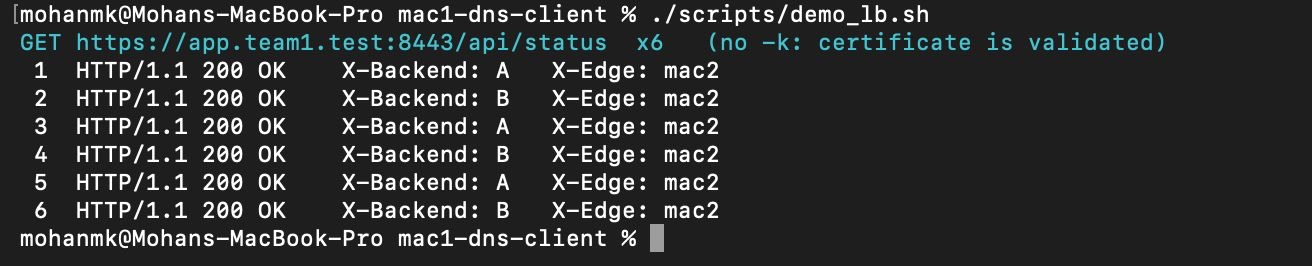
\includegraphics[width=0.62\textwidth]{figures/demo-lb.jpg}
\caption{Load-balancing gate on Mac~1: six HTTPS requests by name with the certificate validated,
alternating between Backend A and Backend B (Listing~\ref{lst:lb}).}
\label{fig:lb}
\vspace{8pt}
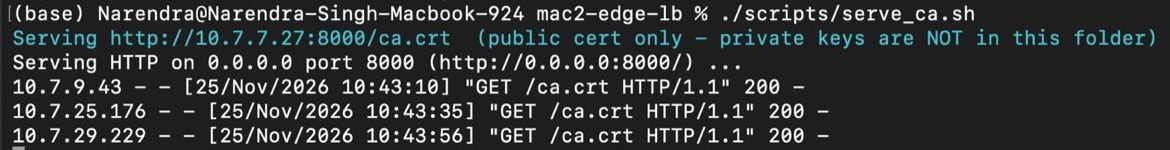
\includegraphics[width=0.66\textwidth]{figures/ca-downloads.jpg}
\caption{CA distribution on Mac~2: only the public certificate is served, and the log records one
download by each client (10.7.9.43, 10.7.25.176, 10.7.29.229).}
\label{fig:ca}
\vspace{8pt}
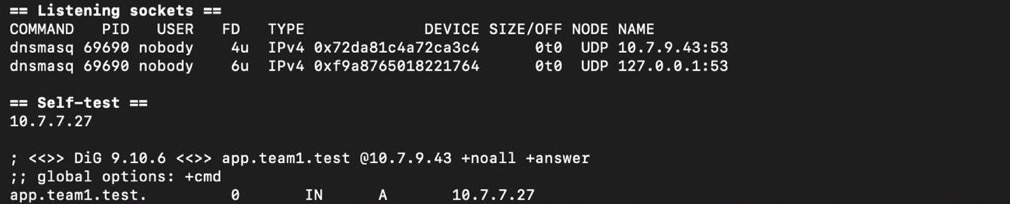
\includegraphics[width=0.6\textwidth]{figures/dnsmasq-selftest.jpg}
\caption{Primary DNS on Mac~1: listening sockets on UDP/53 and a self-test returning the edge
address (Listing~\ref{lst:selftest}).}
\label{fig:dnsmasq}
\end{figure*}

\begin{figure*}[!t]
\centering
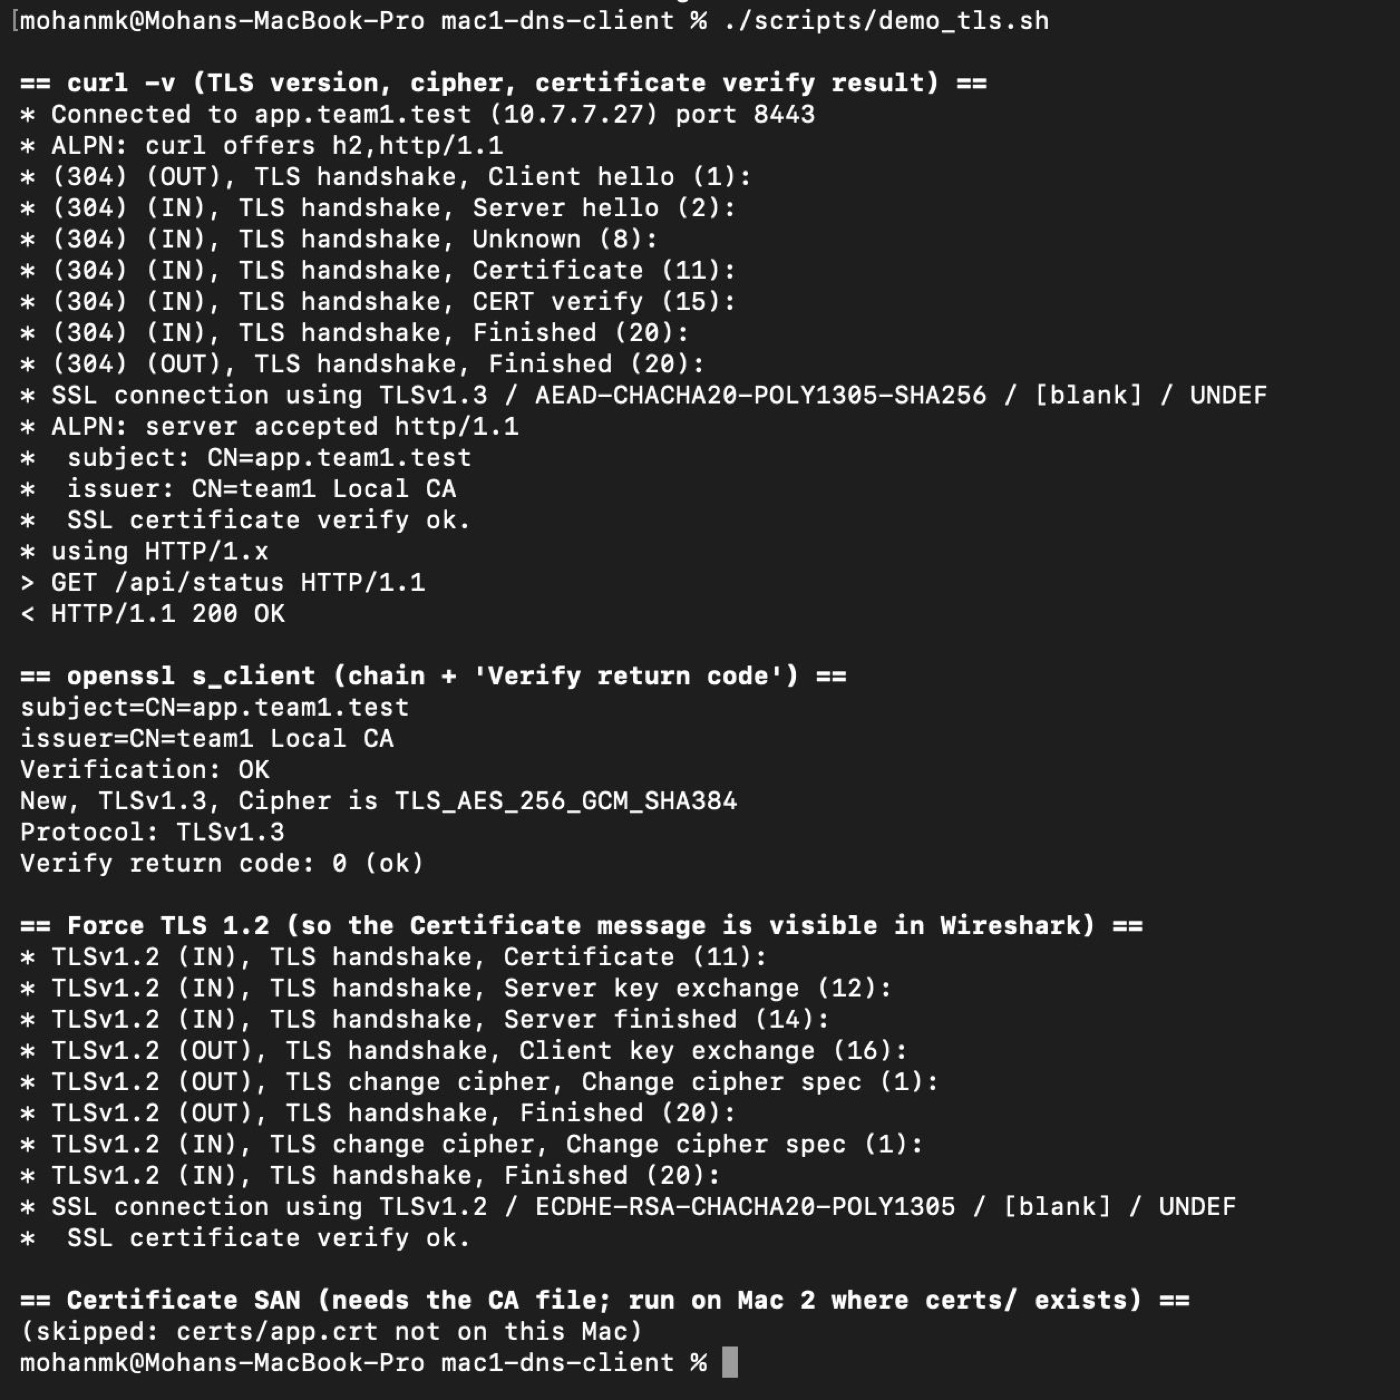
\includegraphics[width=0.5\textwidth]{figures/p1-17-mac1-demo-tls.jpg}
\caption{TLS verification on Mac~1: TLS~1.3 handshake, certificate subject and issuer, successful
verification by curl and OpenSSL, and the forced TLS~1.2 handshake (Listing~\ref{lst:tls}).}
\label{fig:tls}
\end{figure*}

\begin{figure*}[!t]
\centering
\begin{minipage}[b]{0.49\textwidth}\centering
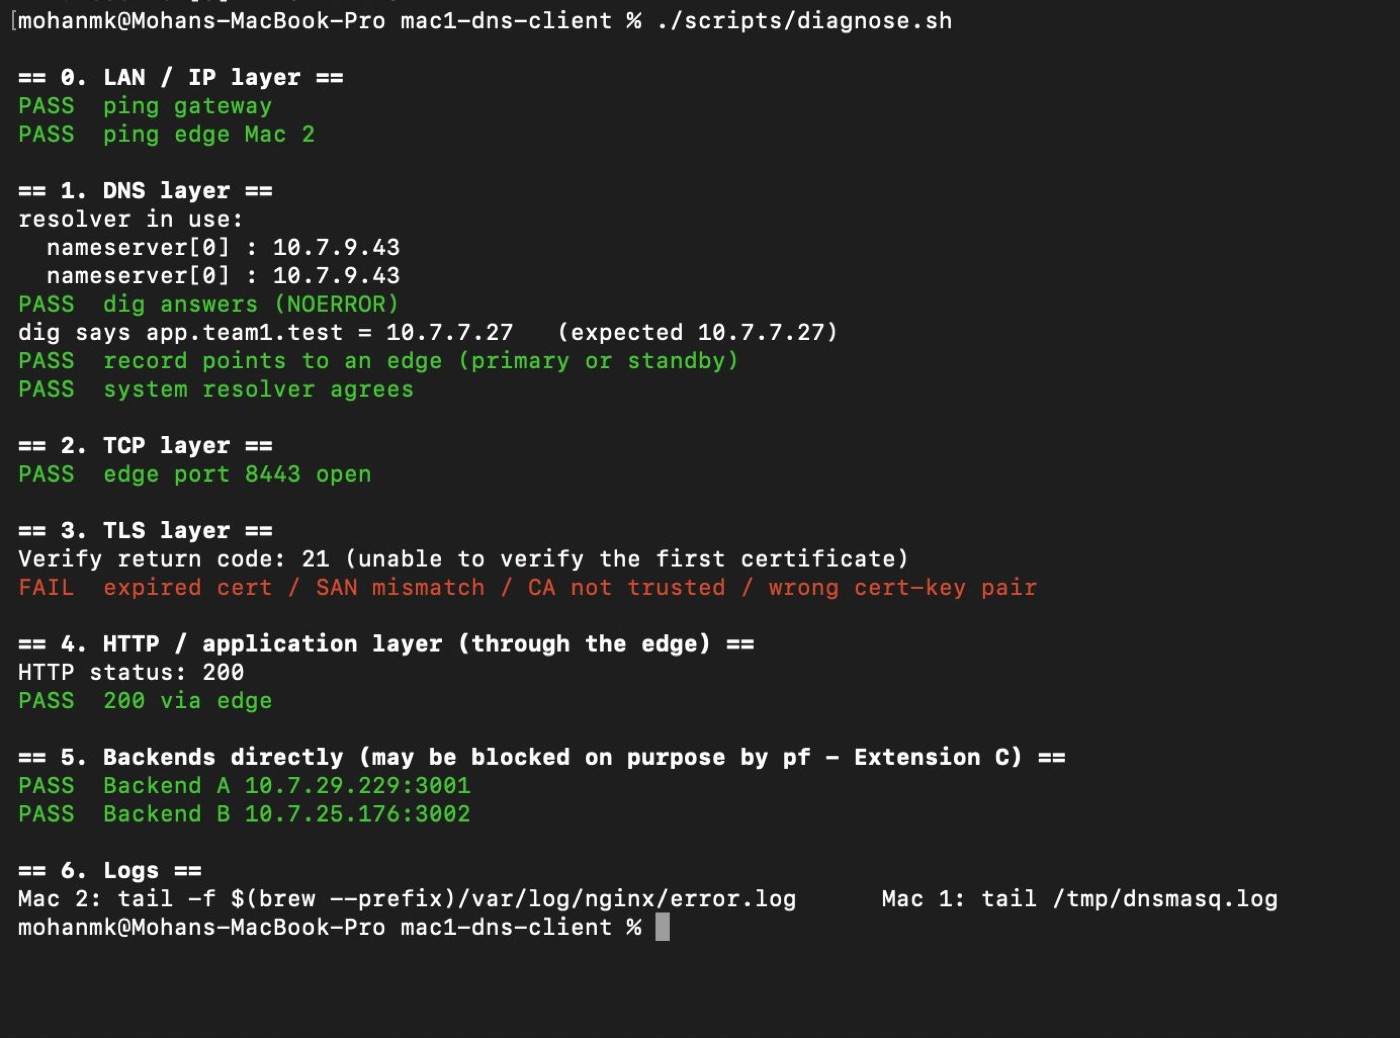
\includegraphics[width=\linewidth]{figures/p1-14-mac1-diagnose-false-fail.jpg}\\[2pt]
{\footnotesize (a) First run: false TLS failure, HTTP passes}
\end{minipage}\hfill
\begin{minipage}[b]{0.49\textwidth}\centering
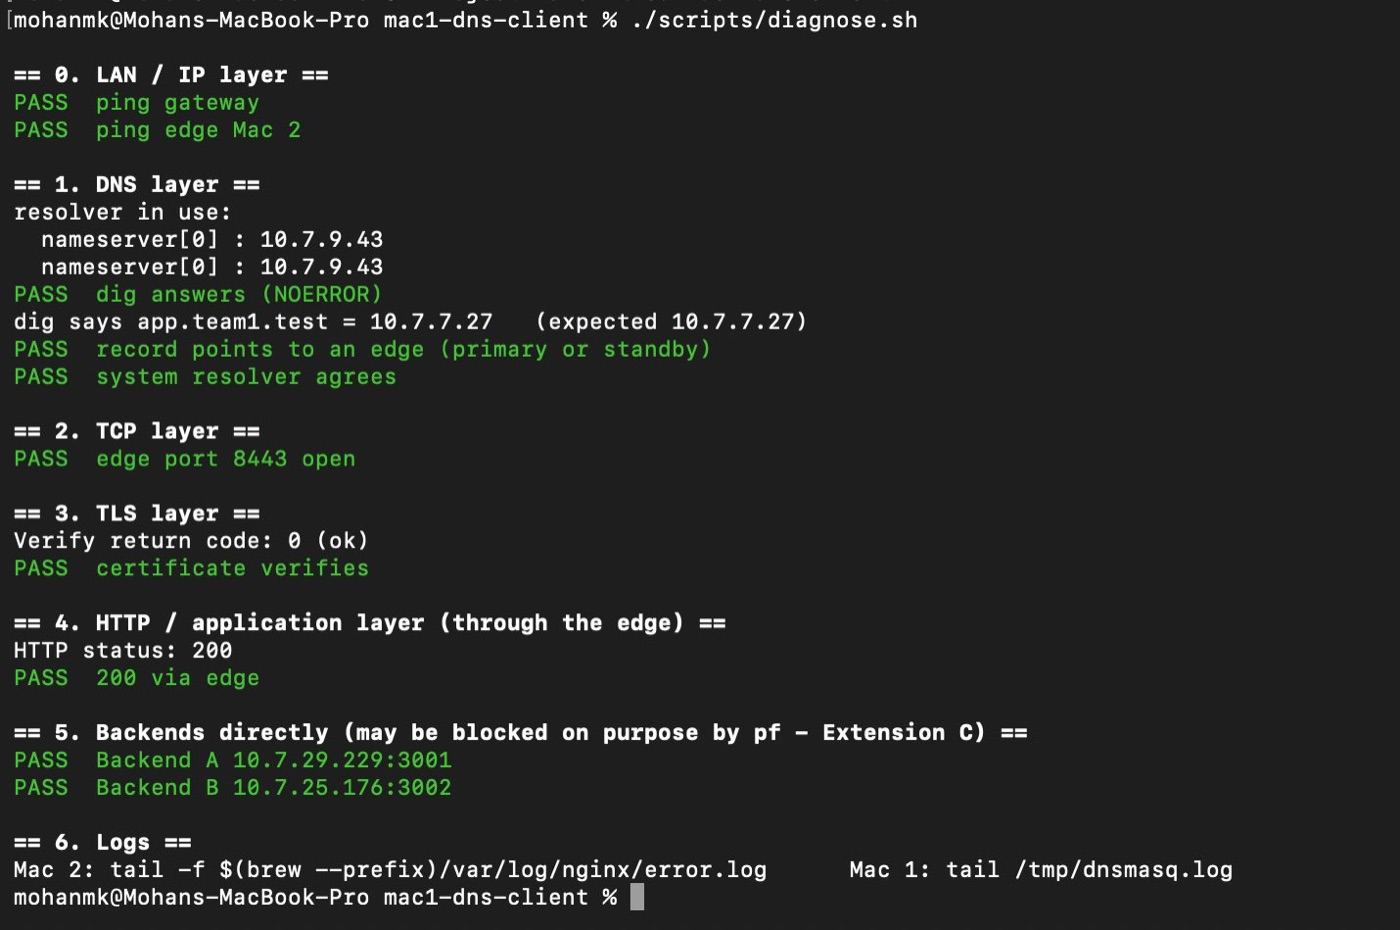
\includegraphics[width=\linewidth]{figures/p1-15-mac1-diagnose-all-pass.jpg}\\[2pt]
{\footnotesize (b) After the \code{-CAfile} fix: all layers pass}
\end{minipage}
\caption{Layered diagnosis on Mac~1 before and after correcting the TLS check
(Listing~\ref{lst:falsefail}).}
\label{fig:diagpair}
\end{figure*}

\end{document}
